\section{Your first Laplace Transform calculations}

\subsection*{Resources}
\begin{itemize}
    \item Videos: The \textbf{four} Khan-academy videos starting at \url{https://www.khanacademy.org/math/differential-equations/laplace-transform/laplace-transform-tutorial/v/laplace-transform-1} % 8m+7:30+10+9 = 35:30
    \item Text (student suggestion, Thai language): \url{http://facstaff.swu.ac.th/surachap/documents/mathematic_i_chapter_3.pdf}
\end{itemize}

\subsection*{Comment}
The Laplace Transform is a powerful technique that has many uses beyond solving ODE's. It can however appear a bit abstract at first. Becoming comfortable with controlling and manipulating the transform will help provide confidence when using it to solve ODE's. The four videos in the resources above provide an excellent starting point for getting you comfortable with this powerful technique.

\subsection*{Challenge}
1. Calculate $\lap{1}$

(2. \emph{Moved to challenge \ref{sec:3rdderiv}})

3. Calculate $\lap{Cos(at)}$

\subsection*{Solution}
To check your answer, substitute $s=1$ and $a=2$ into your final solution.

1. 1

3. $\frac{1}{5}$




%%%%%%%%%%%%%%%%%%%%%%%%%%%%%%%%
\newpage
%%%%%%%%%%%%%%%%%%%%%%%%%%%%%%%%
\section{Laplace transform and derivatives}
\label{sec:3rdderiv}

\subsection*{Resources}
\begin{itemize} % Total video time: 20m
    \item Video I: \url{https://www.khanacademy.org/math/differential-equations/laplace-transform/properties-of-laplace-transform/v/laplace-transform-5} % 11:30
    \item Video II: \url{https://www.khanacademy.org/math/differential-equations/laplace-transform/properties-of-laplace-transform/v/laplace-transform-6} % 9:30
\end{itemize}

\subsection*{Challenge}
1. Calculate $\displaystyle \frac{d^3}{dt^3} \left( t e^{a t} \right)$

2. Given
\begin{equation}
    \lap{t e^{a t}} = \frac{1}{(a-s)^2}
\end{equation}
determine $\lap{3a^2 e^{at} + a^3te^{at}}$

3. Calculate $\lap{at}$\\
Notes:
\begin{itemize}
    \item \emph{L'H\^opital's rule cannot be applied to this question - if you don't understand why, please ask your partner or the teacher in class.}
    \item \emph{You may be able to solve this considering the rate of increase of $e^t$ vs the rate of increase of $t$ as $t$ approaches $\infty$, however there is another way using the relation of derivatives of the Laplace transform, and I would encorage you to understand how to solve it this way.}
\end{itemize}

\subsection*{Solution}
2.\\
If you substitute $s=3$ and $a=2$ into your final solution you should obtain $20$.

3.\\
If you substitute $s=1$ and $a=2$ into your final solution you should obtain $2$.






%%%%%%%%%%%%%%%%%%%%%%%%%%%%%%%%
\newpage
%%%%%%%%%%%%%%%%%%%%%%%%%%%%%%%%
\section{Shifting a transform}

\subsection*{Resources}
\begin{itemize}
    \item Video: \url{https://www.khanacademy.org/math/differential-equations/laplace-transform/properties-of-laplace-transform/v/more-laplace-transform-tools} %11m
\end{itemize}

\subsection*{Challenge}
Given
\begin{equation}
    \lap{Cosh(at)} = \frac{s}{s^2-a^2}
\end{equation}

1. What is $\lap{e^{3t} Cosh(5t)}$?

2. What is $f(t)$ in the equation $\lap{f(t)} = \frac{s-4}{(s-4)^2-100}$?

\subsection*{Solution}
To check your answer, substitute $s=2$ and $t=1/2$ as appropriate:

1. $0.0417$

2. $548$




\stepcounter{section}
%%%%%%%%%%%%%%%%%%%%%%%%%%%%%%%%
%\newpage
%%%%%%%%%%%%%%%%%%%%%%%%%%%%%%%%
%\section{L'H\^opital's rule}
%\label{sec:lopital}
%
%\subsection*{Resources}
%\begin{itemize}
    %\item Wikipedia: \url{https://en.wikipedia.org/wiki/L\%27H\%C3\%B4pital\%27s_rule}
%\end{itemize}
%
%\subsection*{Challenge}
%1. Use L'H\^opital's rule to determine the limit of
%\begin{equation}
    %t e^{-st}
%\end{equation}
%as $t \rightarrow 0$.
%
%2. Considering the case of
%\begin{equation}
    %\frac{t^n}{e^{st}}
%\end{equation}
%if we apply L'H\^opital's rule $n$ times with respect to $t$, what is the power of $t$ in the numerator? Note that $e^{st}$ is always constant, so by repeated differentiation we can apply L'H\^opital's rule even for $t^n$.
%
%\subsection*{Solution}
%1.\\
%\solint{w}{ac1052}
%
%2.\\
%\solint{x}{e50eb7}




%%%%%%%%%%%%%%%%%%%%%%%%%%%%%%%%
\newpage
%%%%%%%%%%%%%%%%%%%%%%%%%%%%%%%%
\section{Laplace Transformation of the unit step function}

\subsection*{Resources}
\begin{itemize}
    \item Video: \url{https://www.khanacademy.org/math/differential-equations/laplace-transform/properties-of-laplace-transform/v/laplace-transform-of-the-unit-step-function} % 24m
\end{itemize}

\subsection*{Challenge}
Considering $U_c$ as the unit step-function at $c$, calculate the following Laplace transformations:

1. $\displaystyle \lap{U_0}$

2. $\displaystyle \lap{U_c}$

3. A 1-second pulse function starting at time $t=1$ with value $f(t)=1$ as shown in the graph below:
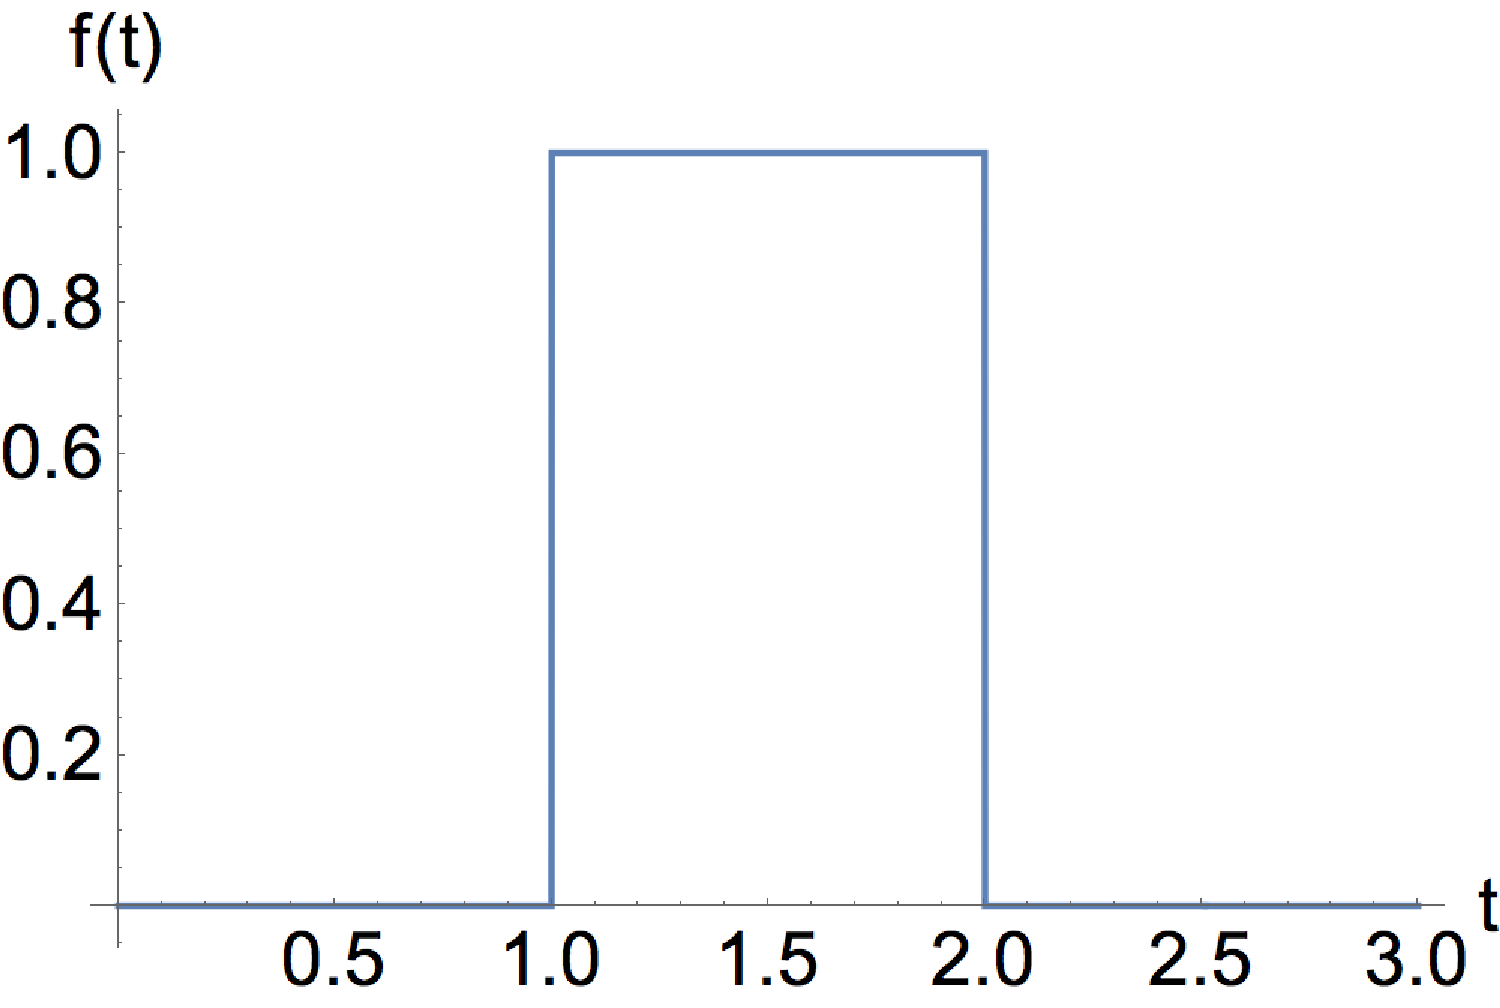
\includegraphics[scale=0.5]{pulse.png}

4. $\displaystyle \lap{U_\pi(t) cos(t-\pi)}$

\subsection*{Solution}
To check your answers, substitute $c=1$ and $s=2$ as appropriate.

1.\\
\soltwodp{y}{4f9ac8}

2.\\
0.0677

3.\\
0.0585

4.\\
\num{7.470e-4}




%%%%%%%%%%%%%%%%%%%%%%%%%%%%%%%%
\newpage
%%%%%%%%%%%%%%%%%%%%%%%%%%%%%%%%
\section{Inverse Laplace Transform}

\subsection*{Resources}
\begin{itemize}
    \item Video: \url{https://www.khanacademy.org/math/differential-equations/laplace-transform/properties-of-laplace-transform/v/inverse-laplace-examples} % 19m
\end{itemize}

\subsection*{Comment}
Being able to reversing the Laplace transform is a crucial skill required for applying it to solving ODE's. It can be a little confusing at first however, so I recommend to take your time to understand the essential steps involved thoroughly, as this will then give you greater confidence when you come to apply this to solving ODE's. To this end, the video listed in the resource is a fantastic introduction to this.

Also, it can be helpful to remember that if you're shifting the transform, perform the transform and \emph{then} apply the shift.

\subsection*{Challenge}
Determine the function $f(t)$ by finding the inverse of the following Laplace transforms:

1. $\displaystyle F(s)=\frac{1}{(s-1)^2}$

2. $\displaystyle F(s)=\frac{1}{s^2} - \frac{1}{s}$

%3. $\displaystyle F(s)=\frac{1-s}{s^2}$

3. $\displaystyle F(s)=\frac{5-5s}{s^2}$

4. $\displaystyle F(s)=\frac{6}{(2+s)^4}$

%5. $\displaystyle F(s)=\frac{120+6s^3}{s^6}$

5. $\displaystyle F(s)=\frac{2 e^{-2s}}{s^2-2s+2}$

6. $\displaystyle F(s)=\frac{e^{12-3s}}{s-4}$

\subsection*{Solution}
To check your answers, substitute $t=2$ into your final answer. If there is a unit-step in your solution, precede your numerical answer with ``u(c)'' where ``c'' is the position of the unit step. So for example, an answer of $U_5 t^2$ with a hash key of ``a'' would be entered as ``au(5.00)4.00'' (all numbers to two decimal places). An answer without a unit-step would just be entered to two decimal places (eg, ``a4.00'' in the previous example).

1.\\
\soltwodp{z}{de950a}

2.\\
\soltwodp{a}{a1e88c}

%3.\\
%\soltwodp{b}{1175d1}

3.\\
\soltwodp{c}{ae77f2}

4.\\
\soltwodp{c}{af01f2}

%5.\\
%\soltwodp{d}{d79888}

5.\\
\soltwodp{b}{b27f51}

6.\\
\soltwodp{e}{cbc74a}



%%%%%%%%%%%%%%%%%%%%%%%%%%%%%%%%
\newpage
%%%%%%%%%%%%%%%%%%%%%%%%%%%%%%%%
\section{The Dirac delta function and its Laplace transform}

\subsection*{Resources}
\begin{itemize}
    \item Video I: \url{https://www.khanacademy.org/math/differential-equations/laplace-transform/properties-of-laplace-transform/v/dirac-delta-function}
    \item Video II: \url{https://www.khanacademy.org/math/differential-equations/laplace-transform/properties-of-laplace-transform/v/laplace-transform-of-the-dirac-delta-function}
\end{itemize}

\subsection*{Challenge}
Calculate the following Laplace transforms (treat $c$ as a positive constant):

1. $\displaystyle \lap{\delta(t)}$

2. $\displaystyle \lap{\delta(t-c)}$

3. $\displaystyle \lap{\delta(t-2) \cos(4 t)}$

4. $\displaystyle \lap{\delta(t) (t^2+10)}$

\subsection*{Solution}
To check your solution, set $s=1$ and $c=2$ as appropriate to check your answers. % Took and $t=1$ out after 2017 course.

1.\\
\soltwodp{z}{a78955}

2. $0.135$

3. $-0.020$

4.\\
\soltwodp{c}{c181ec}




%%%%%%%%%%%%%%%%%%%%%%%%%%%%%%%%
\newpage
%%%%%%%%%%%%%%%%%%%%%%%%%%%%%%%%
\section{The Dirac delta function and its inverse Laplace transform}

\subsection*{Challenge}
1. Calculate the following Laplace transform:

$\displaystyle \delta(t-2) \sin(2t)$

2. Calculate the following inverse Laplace transforms assuming they contain a Dirac delta function:

I. $\displaystyle e^{-2s} \sin(2)$

II. $\displaystyle e^{-2s} \sin(4)$

\subsection*{Solution}
2. To check your answer, substitute $t=1$ into the final expression and evaluate the part inside and outside of the Dirac delta function separately. So for example, if your answer is $\delta(t-2) (t^2+1)$, the expression inside the delta-function is $t-2$ and will evaluate to $-1.00$ while the expression outside of the delta-function is $t^2+1$ and will evaluate to $2.00$.

I. Inside delta function:\\
\soltwodp{d}{4881ba}

I. Outside delta function\\
\soltwodp{e}{724c45}

II. Inside delta function:\\
\soltwodp{f}{75d06e}

II. Outside delta function:\\
\soltwodp{g}{fca71c}




%%%%%%%%%%%%%%%%%%%%%%%%%%%%%%%%
\newpage
%%%%%%%%%%%%%%%%%%%%%%%%%%%%%%%%
\section{A forced spring}

\begin{itemize}
    \item The \textbf{four} videos starting at \url{https://www.khanacademy.org/math/differential-equations/laplace-transform/laplace-transform-to-solve-differential-equation/v/laplace-transform-to-solve-an-equation}
    \item A useful table of Laplace transforms: \url{http://tutorial.math.lamar.edu/pdf/Laplace_Table.pdf}
\end{itemize}

\section*{Comment}
Here you finally get the opportunity to practise solving ODE's using the powerful method of Laplace transformations. Please takes notes from all four videos listed in the resources section; they provide very useful examples of how to use this method, including related algebraic techniques that are commonly required to solve such challenges.

\subsection*{Challenge}
The spring equation you encountered in challenge \ref{sec:hooke} introduced you to the concept of oscillation of a mass on a spring. There, the equation to determine the displacement of the spring $y$ from its equilibrium position was $y''+y=0$, which yields a solution $y=C_1 \cos(t) + C_2 \sin(t)$. This is free oscillation without external damping or driving, and it will oscillate according to the cosine and sine sum for all time ($t$). It is also possible to add a forcing term to the equation by making it non-homogeneous, such as in the form

\begin{equation}
    y'' + 4y = 2 \cos(3t)
\end{equation}

Here the forcing varies with time $t$ in the form of a cosine wave.

Use the Laplace transform method to solve the ODE in the above equation given a starting displacement of zero and an initial velocity of zero. You may use the table of Laplace transforms in the resources to help you.

A graph of the resulting oscillation is shown here:\\
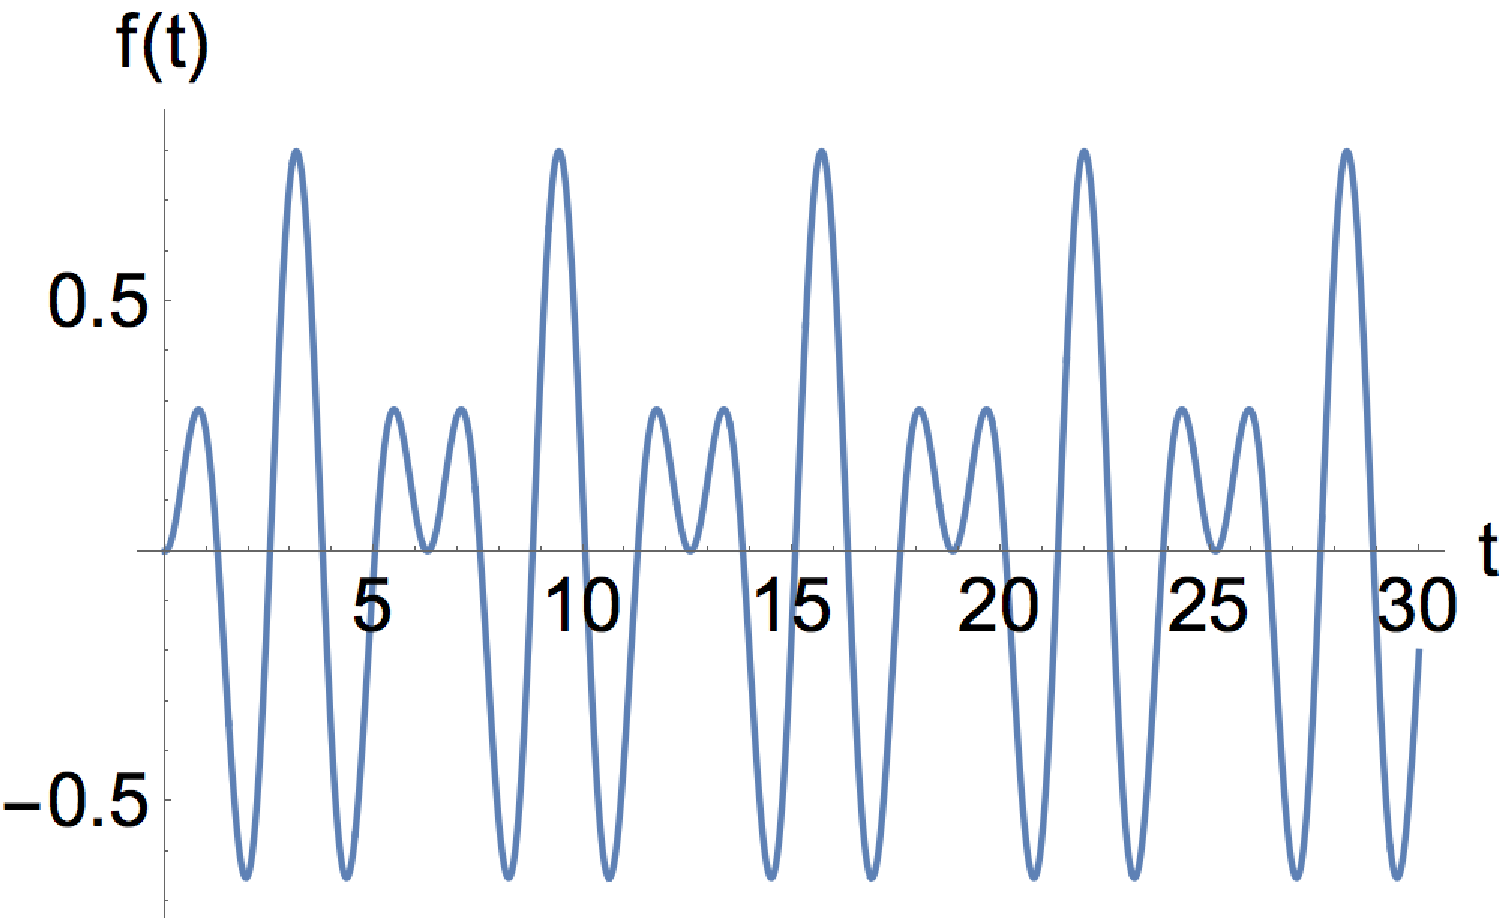
\includegraphics[width=10cm]{cosforcing.png}

\subsection*{Solution}
Your final expression should satisfy $y(t=1)=0.2295$.




%%%%%%%%%%%%%%%%%%%%%%%%%%%%%%%%
\newpage
%%%%%%%%%%%%%%%%%%%%%%%%%%%%%%%%
\section{An exponential function}

\subsection*{Challenge}
1. Solve

\begin{equation}
    y''+5y'+4y=100e^{-2t}
\end{equation}

for $y$, given initial conditions $y(0)=-1$ and $y'(0)=0$. Since the algebra gets very messy, you may use the following equation to help you:
\begin{equation}
    \frac{-s^2-7s+90}{(s+1)(s+2)(s+4)} = \frac{32}{s+1} - \frac{50}{s+2} + \frac{17}{s+4}
\end{equation}

2. The homogeneous solution to this equation is
\begin{equation}
    y(t)= \frac{1}{3} \left( e^{-4t} - 4 e^{-t} \right)
\end{equation}
Show how the two graphs of the homogeneous and non-homogenous solutions differ, and explain how the forcing leads to the different shape observed.

\subsection*{Solution}
1. Your final expression should satisfy $y(1)=5.32$.

2. Please compare your answer with your partner in class or discuss with the teacher.




%%%%%%%%%%%%%%%%%%%%%%%%%%%%%%%%
\newpage
%%%%%%%%%%%%%%%%%%%%%%%%%%%%%%%%
\section{A unit step}

\subsection*{Comment}
There are two things to watch out for in this challenge:
\begin{itemize}
    \item We have defined the Laplace transform for a step function in the sense of $U_c f(t-c)$. So if $f(t)=t$ we must evaluate for $f(t-c)=t-c$. If the function does not contain $t$ then we simply do not need to subtract $c$.
    \item The ``$t-c$'' is essentially substituted in place of any $t$ in the equation. So ``$at$'' will become $a(t-c)$ and not $at - c$.
\end{itemize}

This challenge is interesting because unlike previous challenges, it is the first challenge where we really have no other option but to use the Laplace transform method, and so you can appreciate its power. In this challenge, we have a 2nd-order homogeneous equation (unforced oscillation) until $t=5$ when we apply a constant force. You will find your answer leads to a constant oscillation. But how can it lead to a constant oscillation if we are constantly applying a force? Shouldn't the oscillation slowly increase in magnitude due to the energy that is being added to the system from the constant force being applied? The answer is of course no: we take just as much energy out of the system when the velocity is in the opposite direction to the force as we add to the system when the velocity is in the same direction as the applied force.

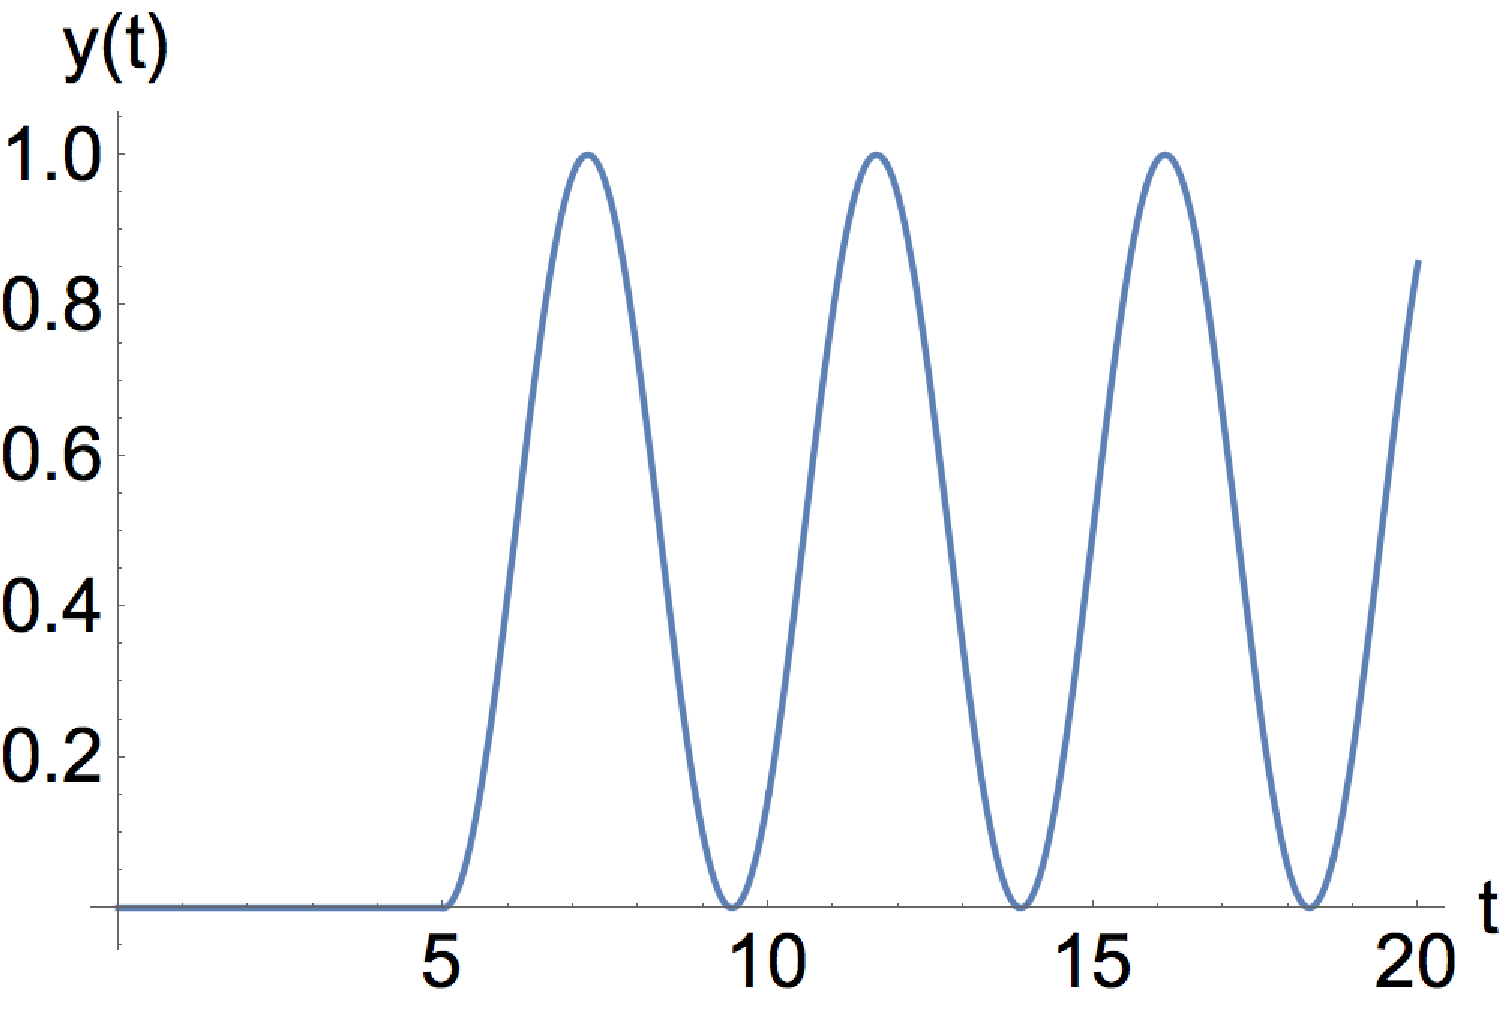
\includegraphics[width=8cm]{stepforcing.png}

\subsection*{Challenge}
Solve

\begin{equation}
    y''+2y=U_5
\end{equation}

for $y$, given initial conditions $y(0)=0$ and $y'(0)=0$. 

\subsection*{Solution}
Your final expression should satisfy $y(t=6)=0.42$.

Note that for $t<5$, the solution is zero. This is because there was no initial velocity and no initial acceleration, so there was no motion until a forcing was applied in terms of a constant force of ``1'' from $t=5$. If either of these had been non-zero, we would have had a non-zero value for $t<5$!

Optionally, you can try setting the initial conditions to non-zero values to see the effect this has on the final solution.



%%%%%%%%%%%%%%%%%%%%%%%%%%%%%%%%
\newpage
%%%%%%%%%%%%%%%%%%%%%%%%%%%%%%%%
\section{A sudden impulse}

\subsection*{Comment}
Here the system is stationary until $t=5$ when, instead of applying a constant force, we ``kick'' the system to start the oscillation. Thus you should expect your answer to reflect physics such as this.

A hint for doing the inverse Laplace transform in this challenge: you will need to multiply the transform by a constant in order to obtain the inverse transform. Also, the graph below should give you a strong indication as to the form of the solution.

\subsection*{Challenge}
Solve

\begin{equation}
    y''+2y=\delta(t-5)
\end{equation}

for $y$, given initial conditions $y(0)=0$ and $y'(0)=0$. 

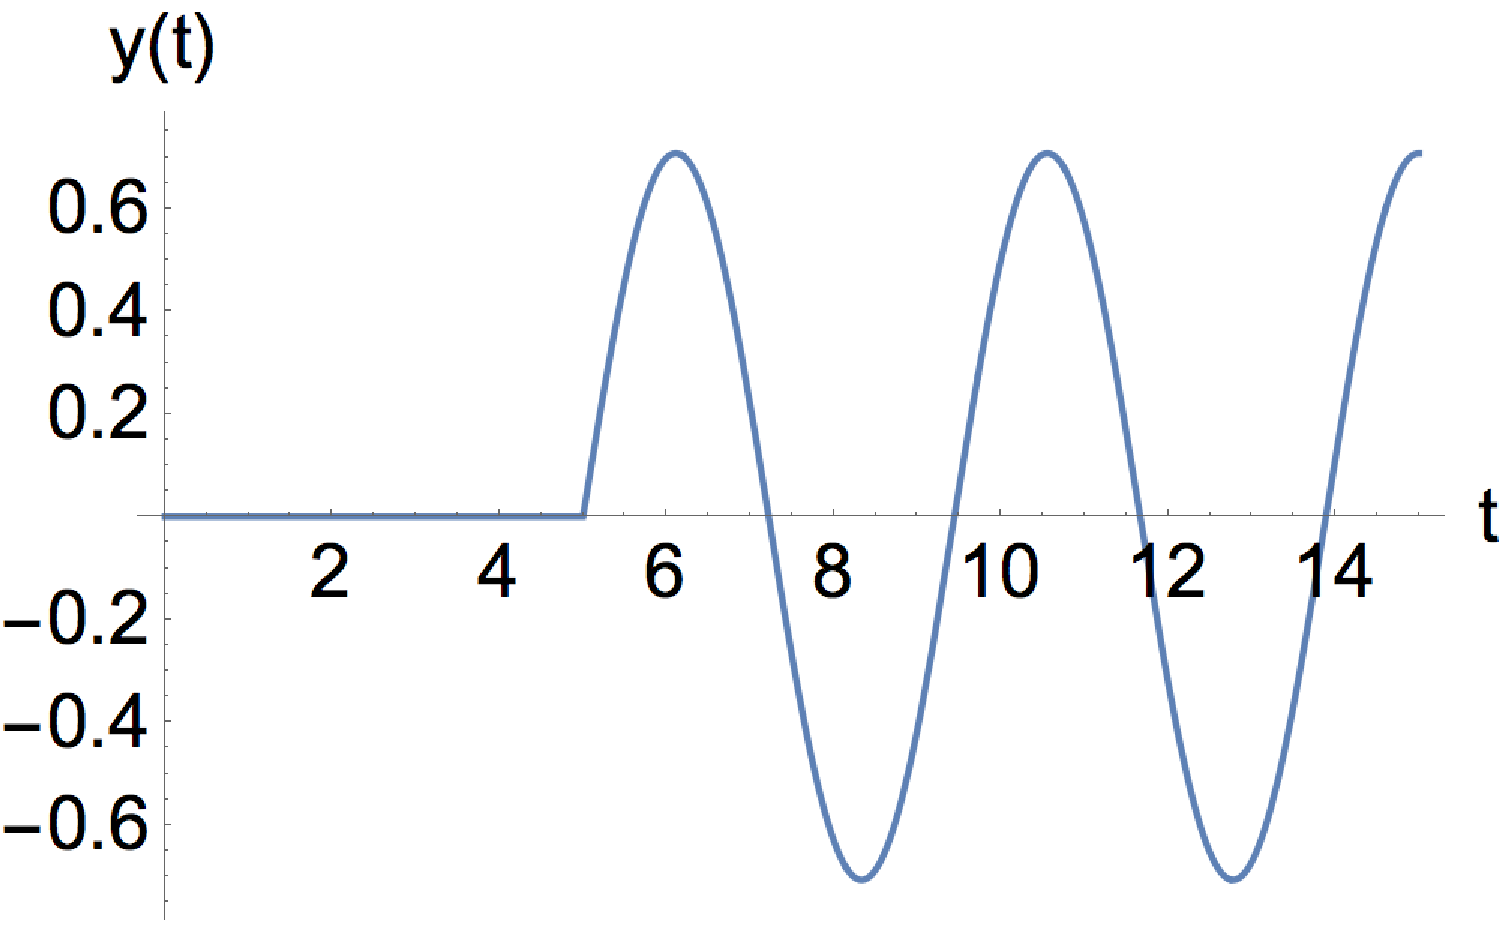
\includegraphics[width=8cm]{deltaforcing.png}

\subsection*{Solution}
Your answer should satisfy $y(6)=0.698$.

Note how this gives rise to a simple oscillation after $t=5$, and nothing before it.




%%%%%%%%%%%%%%%%%%%%%%%%%%%%%%%%
\newpage
%%%%%%%%%%%%%%%%%%%%%%%%%%%%%%%%
\section{Introduction to convolution}

\section*{Resources}
\begin{itemize}
    \item Video \url{https://www.khanacademy.org/math/differential-equations/laplace-transform/convolution-integral/v/introduction-to-the-convolution}
\end{itemize}

\section*{Comment}
In our final study of the application of Laplace transform to solving ODE's, we will look at convolution. This is partly because this is a useful technique for solving ODE's, but also because it will be good for you to have a first-encounter with convolution. So while we are focusing on using Laplace transform and convolution to solve ODE's, my hope is that your familiarity with these topics in this context will make future related topics in other contexts more accessable.

\section*{Challenge}
Evaluate the following expressions:

1. $y(t) = \sin t * \cos t$

2. $y(t) = t * \cos t$

3. $y(t) = 1 * \cos t$

\section*{Solutions}
1. Your answer should satisfy $y(0.9) = 0.352$

2. Your answer should satisfy $y(0.9) = 0.378$

3. Your answer should satisfy $y(0.9) = 0.783$




%%%%%%%%%%%%%%%%%%%%%%%%%%%%%%%%
\newpage
%%%%%%%%%%%%%%%%%%%%%%%%%%%%%%%%
\section{Convolution and the Laplace transform}

\section*{Resources}
\begin{itemize}
    \item Video \url{https://www.khanacademy.org/math/differential-equations/laplace-transform/convolution-integral/v/the-convolution-and-the-laplace-transform}
\end{itemize}

\section*{Challenge}
Obtain the inverse Laplace transform of the following functions using convolution.

1. $\displaystyle \frac{2s}{(s^2 + 1)^2}$

2. $\displaystyle \frac{1}{s^2 - 2s}$

3. $\displaystyle \frac{1}{s^4 + s^2}$

\section*{Solutions}
1. Your solution should satisfy $y(0.8) = 0.574$

2. Your solution should satisfy $y(0.8) = 1.977$

3. Your solution should satisfy $y(0.8) = 0.826$




%%%%%%%%%%%%%%%%%%%%%%%%%%%%%%%%
\newpage
%%%%%%%%%%%%%%%%%%%%%%%%%%%%%%%%
\section{Using convolution to solve ODE's}

\section*{Resources}
\begin{itemize}
    \item Video \url{https://www.khanacademy.org/math/differential-equations/laplace-transform/convolution-integral/v/the-convolution-and-the-laplace-transform}
\end{itemize}

\section*{Challenge}
Using the Laplace transform and convolution, obtain the function $y(t)$ in the form $y(t) = A(t) * B(t)$ (do not attempt to perform the convolution).

1. $\displaystyle y'' - 4 y = \sin t$, with the initial conditions $y(0) = 0$ and $y'(0) = 0$.

2. $\displaystyle y''' - 3a y'' + 3a^2 y' - a^3 y = 2 t$, with the initial conditions $y(0) = 0$, $y'(0) = 0$ and $y''(0) = 0$.

3. $\displaystyle y'' - 10y + 26 = \cos t \sin t$, with the initial conditions $y(0) = 0$ and $y'(0) = 0$.

\section*{Solutions}

1. Your solution should be consistent with $A(0.8) = 0.717$ and $B(0.8) = 2.376$

2. Substituting $a=4$ into the final solution, your solution should be consistent with $A(0.8) = 0.8$ and $B(0.8) = 12.56$.

3. Your solution should be consistent with $A(0.8) = 0.500$ and $B(0.8) = 39.17$
